\documentclass{ativmatUFRB}
%
\usandoXeLuaLaTeX % -------------------> Esse comando indica que você está 
%                                        usando o `LuaLaTeX` ou o `XeLaTeX` como
%                                        compiladores. Mas, se (ainda) estiver
%                                        usando `pdfLaTeX` deve usar o comando
%                                        `\usandopdfLaTeX`.
%=======================================
% Informações do Título da Lista
%=======================================
\tituloDaLista{Título da Lista} %------> Coloque aqui o título da sua lista.
\prof{Fulado Cicrano de Tal} %---------> Nome do Professor.
\disciplina{Miscelânea} %--------------> Disciplina ministrada (Cálculo I, Funções de uma Variável Complexa, etc).
\curso{Licenciatura em Matemática} %---> Curso onde ministra a disciplina.
\semestre{8} %-------------------------> Semestre que onde está inserida a DISCIPLINA.
\numeroDaLista{I} %--------------------> Número da Lisda de Atividade (colocar números em algarismos romanos).
%=======================================

%%%%%%%%%%%%%%%%%%%%%%%%%%%%%%%%%%%%%%%%%%%%%%%%%%%%%%%%%%%%%%%%%%%%%%%%%%%%%%%
% Início da Lista de Atividade
%%%%%%%%%%%%%%%%%%%%%%%%%%%%%%%%%%%%%%%%%%%%%%%%%%%%%%%%%%%%%%%%%%%%%%%%%%%%%%%
\begin{document} %--------------------------------------------------------------> Início do documento.
%
\titulo %-----------------------------------------------------------------------> Gerar o cabeçalho estilizado (com logo da UFRB).
%                                                                                 Não apagar esse comando!
\begin{atividade} %-------------------------------------------------------------> Início do ambiente para questões!
%
%==============================================================================
\topico{Sequências \& Séries} %-------------------------------------------------> Comando para o primeiro tópico.
%==============================================================================   Deixa o nome da seção sombreado com cinza.

% Questão 01 -------------------------------------------------------------------> Note que as questões são iniciadas com \questao.
\questao Na Figura~\ref{fig:espiral} temos uma espiral formada por semicírculos
cujos centros pertencem ao eixos das abscissas. Se o raio do primeiro 
semicírculo é igual a $1$ e o raio de cada semicírculo é igual a metade do 
semicírculo anterior, determine:

\begin{figure}[!h] %------------------------------------------------------------> Ambiente para figuras.
 \centering %-------------------------------------------------------------------> Centralizando a figura.
 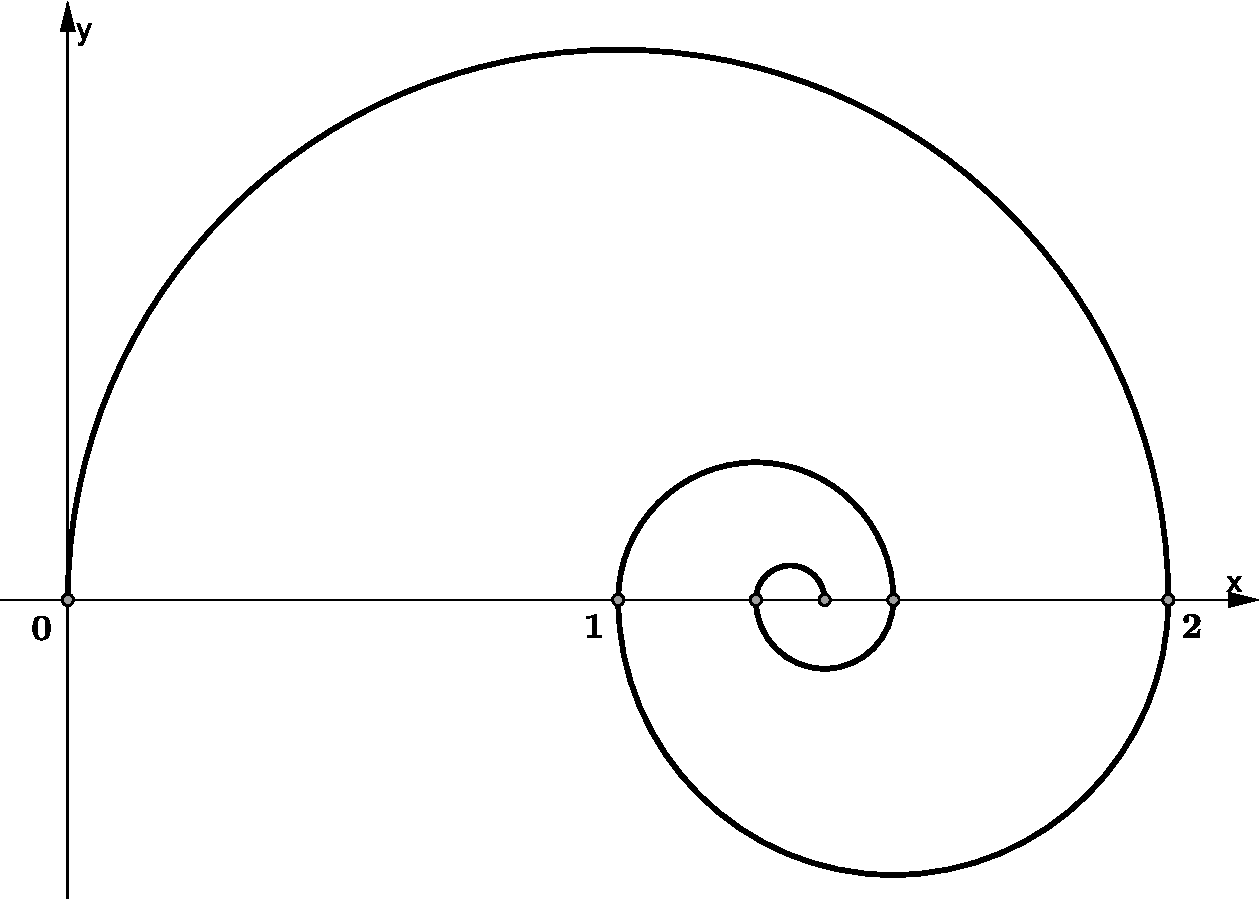
\includegraphics[width=.35\textwidth]{espiral} %-------------------------------> Comando para inserir figura.
 \caption{Um tipo de espiral} %-------------------------------------------------> Legenda da figura.
 \label{fig:espiral} %----------------------------------------------------------> Marcação interna para referências cruzadas.
\end{figure}

\begin{itens} %-----------------------------------------------------------------> Ambiente para listas.
 \item o comprimento da espiral. \Resp{$2\pi$} %--------------------------------> Comando para as respostas.
 \item a abscissa do ponto assintótico da espiral. \Resp{$4/3$}
\end{itens}
%------------------------------------------------------------------------------

% Questão 02 ------------------------------------------------------------------
\questao Uma sequência $(x_n)_{_{n\in\mathbb{N}}}$ é dita \texttt{Sequência de
Cauchy} quando:
\begin{center}
 \fbox
 {
  \begin{minipage}{.7\textwidth}
   Dado arbitrariamente um número real $\displaystyle \varepsilon > 0$, pode-se 
   obter $\displaystyle n_{0}\in \mathbb{N}$ tal que:
   \[
    m > n_{0} \hspace{0.5em} \textrm{ e } \hspace{0.5em} n > n_{0} 
    \Longrightarrow
    \left|x_{m} - x_{n}\right| < \varepsilon.
   \]
  \end{minipage}
 }
\end{center}
\begin{itens}
 \item Mostre que toda sequência convergente é de Cauchy.
\end{itens}
%------------------------------------------------------------------------------

% Questão 03 ------------------------------------------------------------------
\questao Classifique as afirmações abaixo com \textbf{V}~(Verdadeiro) ou 
\textbf{F}~(Falso). Justificando cada uma. Procure justificar as afirmações 
falsas com um contra exemplo.
\begin{multicols}{2} %------------------------------------------------> Ambiente para múltiplas colunas. Nesse caso, colocamos em DUAS colunas.
 \begin{itens}[\vf] %--------------------------------------------------> a opção [\vf] serve para produzir um espaço entre parenteses.
  \item toda sequência decrescente limitada é convergente e seu limite é zero.
  \item toda sequência divergente é não limitada.
  \item toda sequência alternada é divergente.
  \item toda sequência convergente é limitada.
  \item toda sequência limitada é convergente.
  \item toda sequência limitada é monótona.
  \item toda sequência monótona é convergente.
  \item toda sequência divergente é não monótona. 
 \end{itens}
\end{multicols}

%==============================================================================
\topico{Cálculo Vetorial e Integral} %------------------------------------------> Tópico.
%==============================================================================
\subtopico{Integrais Triplas} %-------------------------------------------------> Subtópico.
\subsubtopico{Coordenadas Cilíndricas e Esféricas} %----------------------------> ``Subsubtópico''.

% Questão 04 ------------------------------------------------------------------
\questao Use coordenadas esféricas e calcule as seguintes integrais:

\begin{itens}
 \item 
  $
   \displaystyle
   \int_{-2}^{2}\!
   \int_{-\sqrt{4 - x^2}}^{\sqrt{4 - x^2}}\!
   \int_{\sqrt{x^2 + y^2}}^{\sqrt{8 - x^2 - y^2}}{\left(x^2 + y^2 + z^2\right)\dd z\dd y\dd x}
  $. 
 \Resp{$ \frac{256\pi}{5}\left(\sqrt{2} - 1/2\right) $}
 \item 
  $
   \displaystyle
   \int_{0}^{\sqrt{2}}\!\!
   \int_{y}^{\sqrt{4 - y^2}}\!\!
   \int_{0}^{\sqrt{4 - x^2 - y^2}}{\sqrt{x^2 + y^2 + z^2}\dd z\dd x\dd y}
  $. 
 \Resp{$ \pi $}
\end{itens}
%------------------------------------------------------------------------------
%
\subtopico{Integrais de Linha}
%
% Questão 05 ------------------------------------------------------------------
\questao Seja $\Gamma$ o segmento de reta que liga a origem ao ponto 
$\textrm{A} = (1,1,1)$. 
Calcule $\displaystyle \int_{\Gamma}\vv{F}\dd{\Gamma}$, onde:
\[
 \vv{F}(x,y,z) = xy\versor{i} - y\versor{j} + 1\versor{k}.
\]
%------------------------------------------------------------------------------

%==============================================================================
\topico{Álgebra Linear}
%==============================================================================
\subtopico{Sistemas Lineares}
%
% Questão 06 ------------------------------------------------------------------
\questao (Fuvest-SP-Adap.) Considerando o sistema 
\begin{center}
 \systeme{x+2y+3z=14,4y+5z=23,6z=18}, %---------------------------> Comando para construção de sistemas de equações. 
\end{center}
então o valor de $x$ é igual a:
\altercols{5}{-2}{0}{1}{3}{27} %------------------------------------------------> Comando para múltipla escolha em 5 (cinco colunas).
%------------------------------------------------------------------------------

% Questão 07 ------------------------------------------------------------------
\questao  (IBMEC) Num prédio existem 12 andares, todos ocupados. 
Alguns, por 4 pessoas, outros, por apenas 2 pessoas, num total de 38 pessoas. 
O número de andares ocupados por 2 pessoas é:
\alterdce{4}{5}{6}{8}{19} %-----------------------------------------------------> Comando para múltipla escolha em 2 (duas colunas) fixas.
%------------------------------------------------------------------------------

%==============================================================================
\topico{Estatística}
%==============================================================================

% Questão 08 ------------------------------------------------------------------
\questao Uma pesquisa realizada sobre a preferência dos consumidores por três 
categorias de veículos $A$, $B$ e $C$ de uma indústria automobilística revelou 
que dos 500 entrevistados:

\begin{multicols}{2}
 \begin{itens}[I)]
  \item 210 preferiam o veículo $A$
  \item 230 preferiam o veículo $B$
  \item 160 preferiam o veículo $C$
  \item 90 preferiam o v eículo $A$~e~$B$
  \item 90 preferiam os veículos $A$~e~$C$
  \item 70 preferiam os veículos $B$~e~$C$
 \end{itens}
\end{multicols}

Um consumidor é selecionado ao acaso entre os entrevistados.
Calcule a probabilidade de que:

\begin{itens}
 \item Ele prefira as três categorias.
 \item Ele prefira somente uma das categorias.
 \item Ele prefira apenas a categoria $A$
\end{itens}
%------------------------------------------------------------------------------

% Questão 09 ------------------------------------------------------------------
\questao Cinco corredores foram examinados para determinar a quantidade máxima 
de aspiração de oxigênio, que é uma medida usada para caracterizar a situação 
cardiovascular de uma pessoa.
Os resultados estão na Tabela~\ref{tab:corredor}, onde ``$x$'' é o número de 
segundos no melhor tempo feito em um quilômetro e ``$y$'' é o número de 
mililitros por minuto, por quilograma de peso corporal da aspiração máxima de 
oxigênio do corredor.

\begin{table}[!htbp] %----------------------------------------------------------> Ambiente para Tabela/ Posicionamento no texto.
 \caption{Segundos por melhor corredor} %---------------------------------------> Legendas da tabela.
 \label{tab:corredor} %---------------------------------------------------------> Marcação para referencias cruzadas.
 \centering %-------------------------------------------------------------------> Centraliza a tabela.
 \begin{tabular}{l c c c c c} %---------------------> Tabela estilizada/ Cada letra é uma coluna (c: centralizada; l: à esquerda; r: à direita).
  \toprule %------> Linha superior.
                & \textbf{Corredor A} & \textbf{Corredor B} & \textbf{Corredor C} & \textbf{Corredor D} & \textbf{Corredor E}\\
  \midrule %------> Linha média.
   $\mathbf{x}$ & 300,5               & 350,6               & 407,3               & 326,2               & 512,8\\
   $\mathbf{y}$ & 350,2               & 325,8               & 375,6               & 418,5               & 400,2\\
  \bottomrule %---> Linha inferior.
 \end{tabular}
\end{table}
	
\begin{itens}
 \item Trace o diagrama de dispersão.
 \item Ache a reta de regressão para os dados da tabela.
 \item Use a reta de regressão para estimar a máxima aspiração de oxigênio de um
  corredor, cujo melhor tempo em uma milha é de \unit[340,4]{s}. %--------------> `\unit[]{}` padroniza unid. de media (veja também `siunitx`).
\end{itens}
%------------------------------------------------------------------------------

%==============================================================================
\topico{Variáveis Complexas}
%==============================================================================

% Questão 10 ------------------------------------------------------------------
\questao (UFMS-adap.) Sobre o número complexo $z$ que satisfaz a equação 
\[
 2 \bar{z} + iz + 1 - i = 0,
\]
julgue os itens abaixo em \textbf{V}~(verdadeiro) ou \textbf{F}~(falso).
\begin{multicols}{3}
 \begin{itens}[\vf]
  \item $\displaystyle \left|z\right|=\sqrt{z}$.
  \item $\displaystyle \textrm{Re}\left(z\right)+\textrm{Im}\left(z\right)=0$.
  \item $\displaystyle \bar{z} = -1 + i$.
  \item $\displaystyle z$ é um número real.
  \item $\displaystyle z^{2} = i$.
 \end{itens}
\end{multicols}
%------------------------------------------------------------------------------

% Questão 11 ------------------------------------------------------------------
\questao Sendo $\varphi\colon [0,2\pi]\to\mathbb{C}$, definida por 
$ \varphi(t) = 1 + e^{it} $, tal que $ \Phi = \varphi\left([0,2\pi]\right) $, 
encontre:
\[
 \intc_{\Phi}\frac{1}{z^2-1} \dd{z} %-------------------------------------------> Comando para integral circular com orientação ``positiva''.
\]
de duas formas:
\begin{itens}
 \item Diretamente (usando parametrização).
 \item Usando o \texttt{Teorema da Integral de Cauchy}.
\end{itens} 
%------------------------------------------------------------------------------

% Questão 12 ------------------------------------------------------------------
\questao Prove que
\[
  \sen{\left(\frac{2\pi}{7}\right)} + 
  \sen{\left(\frac{4\pi}{7}\right)} + 
  \sen{\left(\frac{8\pi}{7}\right)} =
  \frac{\sqrt{7}}{2}.
\]
%------------------------------------------------------------------------------
%
\end{atividade}
%
%------------------------------------------------------------------------------
% Fim da Lista de Atividade
%%%%%%%%%%%%%%%%%%%%%%%%%%%%%%%%%%%%%%%%%%%%%%%%%%%%%%%%%%%%%%%%%%%%%%%%%%%%%%%
\end{document}